\section{System Performance}{\label{secSysperf}}
  
Handover means that the system will have passed the NSF and DOE close out review. The as delivered system will be capable of delivering images that satisfy the science requirements as defined in SRD (\cite{LPM-17}). Following the final phase of commissioning which will include science validation (SV) observations, the state of the system will be assessed and the readiness of the system and team to begin the survey will be made. 

Rubin has developed a high level metric to summarize the system performance with respect to survey efficiency. We need to ensure both that the system is producing science capable images and data products and that the observing is efficient. 
If the site and system are producing appropriate image quality and the system and team are acquiring data efficiently coming out of SV, we can confidently start the LSST. In Figure~\ref{fE}, we show the system contribution to image quality (and atmospheric contribution) versus the dimensionless survey efficiency or ``speed,'' fE. 

\begin{figure}%[!ht]
  \centering
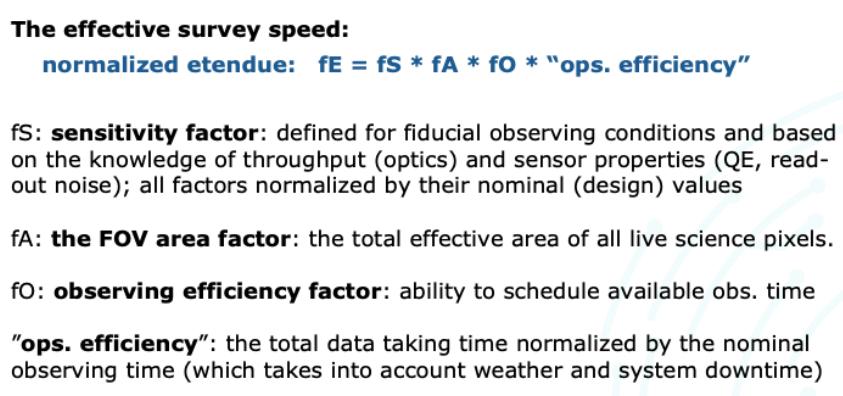
\includegraphics[width=0.75\linewidth]{fE.png}
\caption{Dimensionless survey efficiency factor, fE. Only ops efficiency is not known precisely at this time by data or design. The ComCam run will allow a specific determination of fE as we roll into LSSTCam commissioning. fE will be fully updated by as built system performance and ops. efficiency by the end of science validation.}
\label{fE}
\end{figure}

All f factors are dimensionless and normalized by the corresponding SRD design values. They can be “traded against each other” as “time”.
For example, deterioration in the mirror reflectivity can be easily translated to factor fS, and traded against time (e.g. time lost to recoating, the system “efficiency”), or against loss of sensor area (fA).
The key point is that it is possible to define a simple measurable quantity (fE) that is an excellent numerical approximation for “LSST science goals”. Thus, we can think of the effective speed of executing the LSST (in units of the nominal speed) in terms of recognizable elements: fE ~ ”eff area” * “eff FOV” * “cadence” * “downtime”

In Figure~\ref{speed}, we show the current state of our understanding of the image quality and survey speed.

\begin{figure}[t]
  \centering
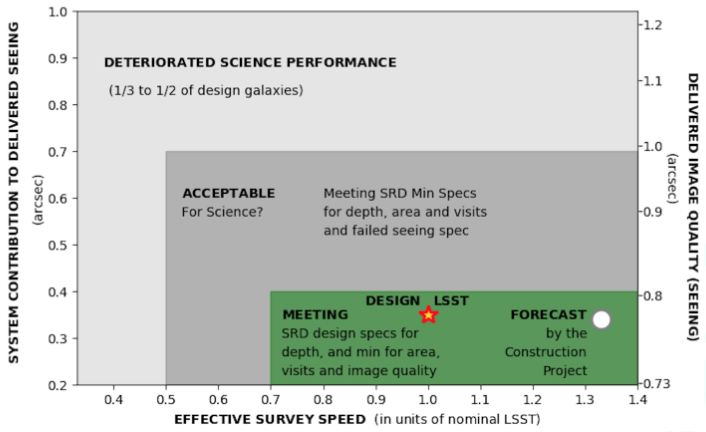
\includegraphics[width=0.85\linewidth]{speed.png}
\caption{Image quality versus effective survey speed, fE. The system contribution to the image quality is shown on the left vertical axis and the delivered image quality including the atmosphere (added in quadrature) is on the right. The LSST design is accomplished with nominal speed 1.0 and system IQ of 0.35$''$ in this diagram. Based on known subsystem performance and design, the current forecast shows the LSST will be accomplished with significant margin. Any final margin will be used to reassess the survey strategy given by \cite{PSTN-056}.}
\label{speed}
\end{figure}

There are three regions in the diagram. Clearly we want to be in the green shaded region and to the lower right in the space. The current understanding og the system as verified through subsystem verification or from the design and median seeing from the free atmosphere (0.7$''$) suggests we are in good shape. Experience with ComCam in late 2024 suggests we should be able to reach high ops efficiency. This will be quantified in the upcoming LSSTCam commissioning period.  


